\documentclass[12pt]{beamer}
%\documentclass[handout,xcolor=pdflatex,dvipsnames,table,12pt]{beamer}
\usepackage[latin1]{inputenc}
%\usepackage[T1]{fontenc}
\usepackage{amsmath} % for math AMS fonts
\usepackage{graphicx} % to include figures
\usepackage{subfigure} % to have figures in figures
\usepackage{multimedia} % to include movies
\usepackage{listings} % to display code
\usepackage{colortbl} % colored tables
\usepackage[latin1]{inputenc} % support for accented letters, etc.
\usepackage{amsthm}
\usepackage{hyperref}
\usepackage{ulem}
\usepackage{booktabs}
\usepackage{tikz}
\usepackage{mathtools}

\usetheme{Warsaw}
\setbeamercovered{invisible}

\title[Introduction to Cryptography]{Homomorphic Encryption}
\author{Christian Mann -- christian-mann@utulsa.edu}
\institute{University of Tulsa\\
Tulsa, Oklahoma 74104}
\date{\today}

\logo{
\includegraphics[height=1.5cm]{pictures/SFSLogoMain}}

\begin{document}

\lstset{
language=python,                % choose the language of the code
%basicstyle=\footnotesize,       % the size of the fonts that are used for the code
%numbers=left,                   % where to put the line-numbers
%numberstyle=\footnotesize,      % the size of the fonts that are used for the line-numbers
%stepnumber=2,                   % the step between two line-numbers. If it's 1 each line will be numbered
%%umbersep=5pt,                  % how far the line-numbers are from the code
%backgroundcolor=\color{white},  % choose the background color. You must add \usepackage{color}
showspaces=false,               % show spaces adding particular underscores
showstringspaces=false,         % underline spaces within strings
showtabs=false,                 % show tabs within strings adding particular underscores
%%frame=single,	                % adds a frame around the code
tabsize=4,	                % sets default tabsize to 2 spaces
%%captionpos=b,                   % sets the caption-position to bottom
%%breaklines=true,                % sets automatic line breaking
%%breakatwhitespace=false,        % sets if automatic breaks should only happen at whitespace
%%title=\lstname,                 % show the filename of files included with \lstinputlisting; also try caption instead of title
%escapeinside={\%*}{*)}          % if you want to add a comment within your code
%morekeywords={*,...}            % if you want to add more keywords to the set
}

\newtheorem{mydef}{Definition}


\begin{frame}
\titlepage
\end{frame}


% no outline

% note, you should have three sections maximum.  two is good.  subsubsections are evil.
% new slides begin with teh \begin{frame} and end with \end{frame}

\iffalse
\fi

\begin{frame}{Homomorphic Encryption}
	\begin{block}{Homomorphic Encryption}
		Homomorphic encryption is a form of encryption that allows computations
		to be carried out on ciphertext, thus generating an encrypted result
		which, when decrypted, matches the result of operations performed on the
		plaintext.
	\end{block}

	\begin{block}{Problem}
		We want to offload computation to another actor, but we don't want to
		let them read our data.
	\end{block}
\end{frame}

\begin{frame}{Homomorphic Encryption}
	\begin{block}{Applications}
		\begin{itemize}
			\item \textbf{Financial} data that needs to be kept secret
			\pause
			\item \textbf{MRI} scan data that needs to be processed
			\pause
			\item \textbf{Snapchat} contact matching
		\end{itemize}
	\end{block}
\end{frame}

\begin{frame}{Description}
	\begin{columns}[c]
		\column{.5\textwidth}
		 \begin{itemize}
		 	\item<1-> Start with message $m$
		 	\item<2-> Encrypt message $m$ to $E(m) = c$
		 	\item<3-> Apply function $g$ to $c$ to get $c'$
		 	\item<4-> Decrypt $c'$ to $D(c') = m'$
		 	\item<5-> Convert (efficiently) $m'$ to $f(m)$
		 \end{itemize}
		\column{.5\textwidth}
		 \begin{tikzpicture}
			 \draw<2-> (0,3) -> (3,3) node [midway, above, fill=white] {$E_K$};
			 \draw<3-> (3,3) -> (3,0) node [midway, right, fill=white] {$g$};
			 \draw<4-> (3,0) -> (0,0) node [midway, above, fill=white] {$D_K$};
			 \draw<5-> (0,0) -> (0,-1);
			 \node<1-> [fill=white] at (0,3) {$m$};
			 \node<2-> [fill=white] at (3,3) {$E_K(m)$};
			 \node<3-> [fill=white] at (3,0) {$g(E_K(m))$};
			 \node<4-> [fill=white] at (0,0) {$m'$};
			 \node<5-> [fill=white] at (0,-1) {$f(m)$};
		 \end{tikzpicture}
	\end{columns}
\end{frame}

\begin{frame}{An Analogy}
	\begin{itemize}
		\item You own a jewelry store
		\item You want your employees to repair jewelry but you don't trust them
		\item Employees work inside locked gloveboxes
	\end{itemize}
	\begin{figure}[h!]
		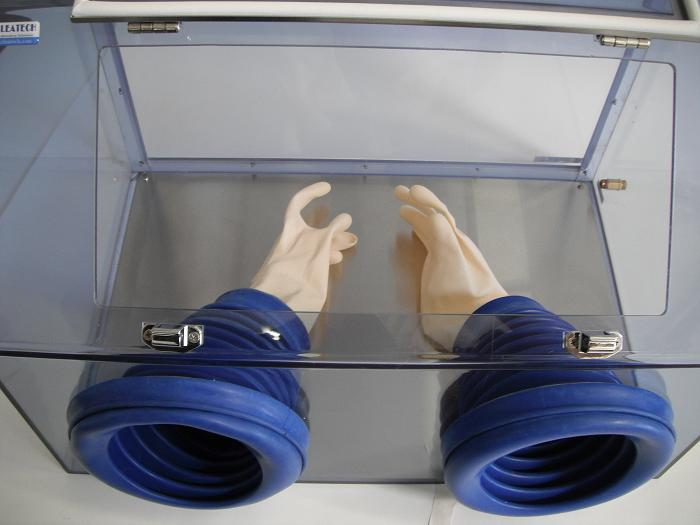
\includegraphics[width=\textwidth, height=.4\textheight, keepaspectratio]{./pictures/glovebox}
		\caption{A glove box.}
	\end{figure}
\end{frame}

\begin{frame}{Malleable Encryption}
	\begin{block}{Hey, wait a minute...}
		ECB, CBC have this property -- ``attacker'' can modify ciphertext
		without decrypting it.
	\end{block}
	
	\begin{block}{Malleability vs Homomorphicity}
		Every homomorphic encryption scheme is malleable in some way. It depends
		on your threat model.

		Confidentiality vs Authenticity
	\end{block}
\end{frame}

\begin{frame}{Unpadded RSA}
	\begin{align*}
		E_K(m) &= m^e \mod n \\
		E_K(m_1 * m_2) &= m_1^e m_2^e \mod n \\
		&= (m_1m_2)^e \mod n \\
		&= E_K(m_1) E_K(m_2)
	\end{align*}

	\begin{block}{}
		So the product of the encryptions is the encryption of the product. The
		``RSA Parity'' lab deals with this.
	\end{block}

	\begin{alertblock}{Problem}
		Unpadded RSA under a static key can be considered a substitution cipher!
	\end{alertblock}
\end{frame}

\begin{frame}{ElGamal Encryption}
	ElGamal is like this: $K_{pub} = (p, g, g^x)$; $K_{priv} = x$;
	\begin{align*}
		r &\xleftarrow{\$} \mathbb{Z}_p \\
		E_K(m) &= (g^r, m(g^x)^r) = (c_1, c_2) \\
		s &= c_1^x = g^{rx} \\
		m' &= c_2s^{-1} = mg^{xr} (g^{rx})^{-1} = m
	\end{align*}
	
	\begin{block}{Randomized Encryption}
		We choose $r$ randomly, which means we can re-use the key.
	\end{block}
\end{frame}

\begin{frame}{ElGamal Encryption is Homomorphic under Multiplication}
	If we take two ciphertexts and multiply them...
	\begin{align*}
		E_K(m_1) \cdot E_K(m_2) &= (g^{r_1}, m_1g^{xr_1}) \cdot
		(g^{r_2}, m_2g^{xr_2}) \\
		&= (g^{r_1}g^{r_2}, m_1g^{xr_1}m_2g^{xr_2}) \\
		&= (g^{r_1+r_2}, m_1m_2g^{x(r_1 + r_2)}) \\
		&= (g^R, m_1m_2g^{xR})
	\end{align*}
	This is a valid encryption of $m_1m_2$.

	\begin{block}{Randomized Encryption}
		Because the $r$ value for the result is different from the originals,
		the server does not know anything about the result.
	\end{block}
\end{frame}

\begin{frame}{Goldwassen-Micali}
	\begin{itemize}
	\item Goldwassen-Micali uses quadratic residuosity.

	\item Private key: $(p, q)$ large primes;
	\item Public key: $(pq, x)$ where $x$ is not a quadratic residue mod $n$
		(i.e. $x \neq y^2$)

	\item We encrypt one bit at a time.
	\end{itemize}

	\begin{align*}
		E_K(b) = x^b r^2 \mod n; r \xleftarrow{\$} \mathbb{Z}_n \\
		D_K(c) = \begin{cases} 0 & c \text{ a square} \\ 1 & c \text{ not a
			square} \end{cases}
	\end{align*}
\end{frame}

\begin{frame}{Goldwassen-Micali homomorphic under XOR}
	If we take two ciphertexts and multiply them...
	\begin{align*}
		E_K(b_1)E_K(b_2) &= x^{b_1}r_1^2 x^{b_2}r_2^2 \mod n \\
		&= x^{b_1 + b_2} (r_1r_2)^2 \\
		&= \begin{cases} (r_1r_2)^2 & b_1 = b_2 = 0 \\
			x (r_1r_2)^2 & b_1 \neq b_2 \\
			(xr_1r_2)^2 & b_1 = b_2 = 1 \end{cases}
	\end{align*}

	When decrypted, this is $b_1 \oplus b_2$.
\end{frame}

\begin{frame}{Fully Homomorphic Schemes}{aka pipe dream}
	\begin{block}{Boolean Circuits}
		Any function $\{0,1\}^a \rightarrow \{0,1\}^b$ can be expressed by a (large)
		Boolean circuit of logic gates.
	\end{block}

	\begin{block}{Universal Gates}
		NAND and NOR can be used to make any circuit -- \{AND, XOR\} works as
		well. You also need ground and power (0 and 1).
	\end{block}

	\begin{block}{Idea}
		If we can just find something that's homomorphic in both XOR and AND (+
		and *), then we have a full homomorphic scheme.
	\end{block}
\end{frame}

\begin{frame}{Lattice-Based Cryptography}{A Fully Homomorphic Scheme}
	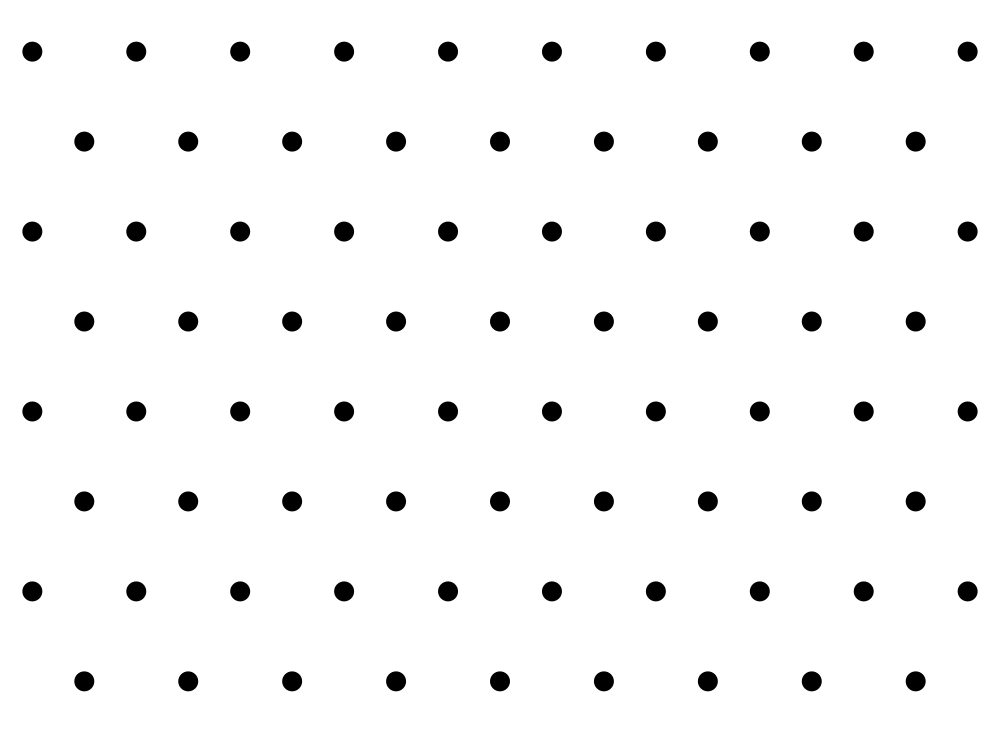
\includegraphics[width=\textwidth]{./pictures/lattice}
\end{frame}

\begin{frame}{Lattice-Based Cryptography}{A Fully Homomorphic Scheme}
	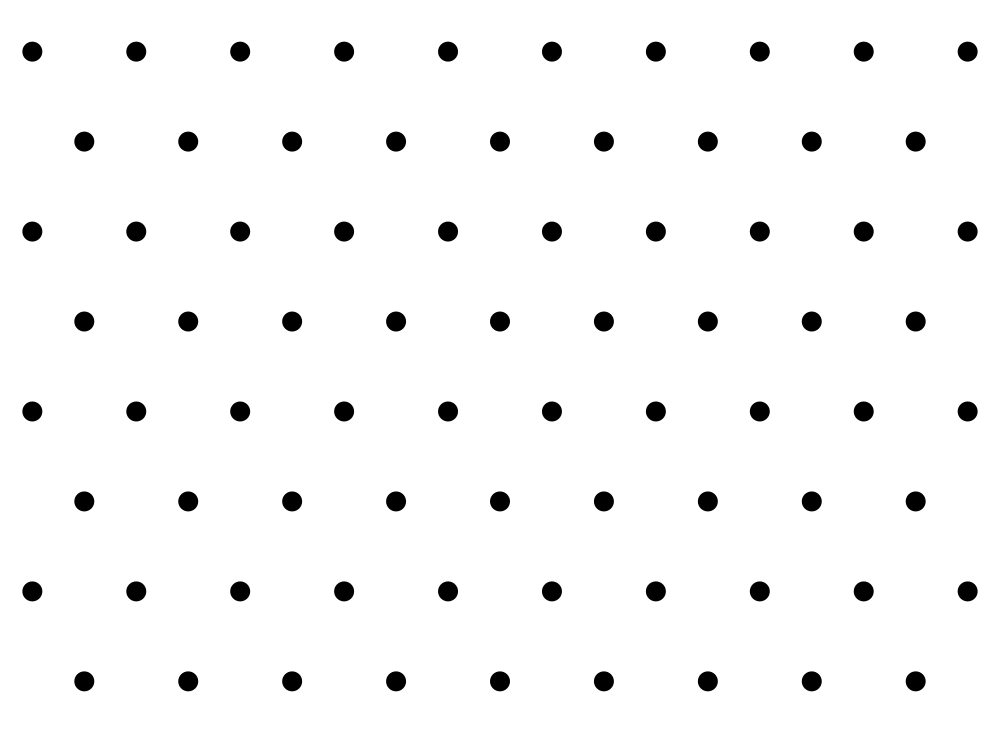
\includegraphics[width=0.3\textwidth]{./pictures/lattice}
	\begin{itemize}
		\item Lattice is expressible in terms of \textit{basis vectors}
		\item More than one basis -- some are hard, some are not
		\item Values are points in $\mathbb{R}^n$
		\item Shortest Vector Problem, Closest Vector Problem
	\end{itemize}
\end{frame}

\begin{frame}{Dealing with Noise}
	\begin{itemize}
		\item Lattice-based crypto gives us ``homomorphic encryption,'' but...
		\item Lattices accumulate errors
		\item Can ruin result after enough computation
	\end{itemize}

	\begin{block}{Craig Gentry, Ph.D.}
		In 2009, Craig Gentry earned his Ph.D. for a scheme that builds an
		error-free scheme out of a scheme with a known error rate. We're going
		to go over the \textit{basic} idea.

		``A Fully Homomorphic Encryption Scheme'', Craig Gentry, 2009. Stanford.
	\end{block}
\end{frame}

\begin{frame}{``Freezing'' Noise in place}
	\begin{block}{Bootstrappable Schemes}
		If a homomorphic encryption scheme is capable of running its own
		decryption circuit without error, it is called \textit{bootstrappable}.
	\end{block}

	Idea: Trade our encrypted data for equivalent, fresh data; i.e. decrypt and
	re-encrypt. Without the secret key we can't decrypt the message, but we can
	\textit{homomorphically}!
	\begin{align*}
		\psi_1 &= \leftarrow E_{K_1}(\pi) \\
		\overline{\psi_1} &\leftarrow E_{K_2}(\psi_1) \\
		\overline{K_1} &\leftarrow E_{K_2}(K_1) \\
		\psi_2 &\leftarrow \text{Evaluate}(K_2, D, \overline{K_1},
		\overline{\psi_1})
	\end{align*}
\end{frame}

\begin{frame}{An Extended Analogy}
	\begin{itemize}
		\item Same jewelry store
		\item Gloves are broken and unusable after one minute
		\item Give multiple gloveboxes
		\item Each has the key to the previous one
		\item After one minute, put glovebox 1 into 2, unlock 1, and continue
	\end{itemize}
\end{frame}

\begin{frame}{The Price of Homomorphic Encryption}{Performance}
	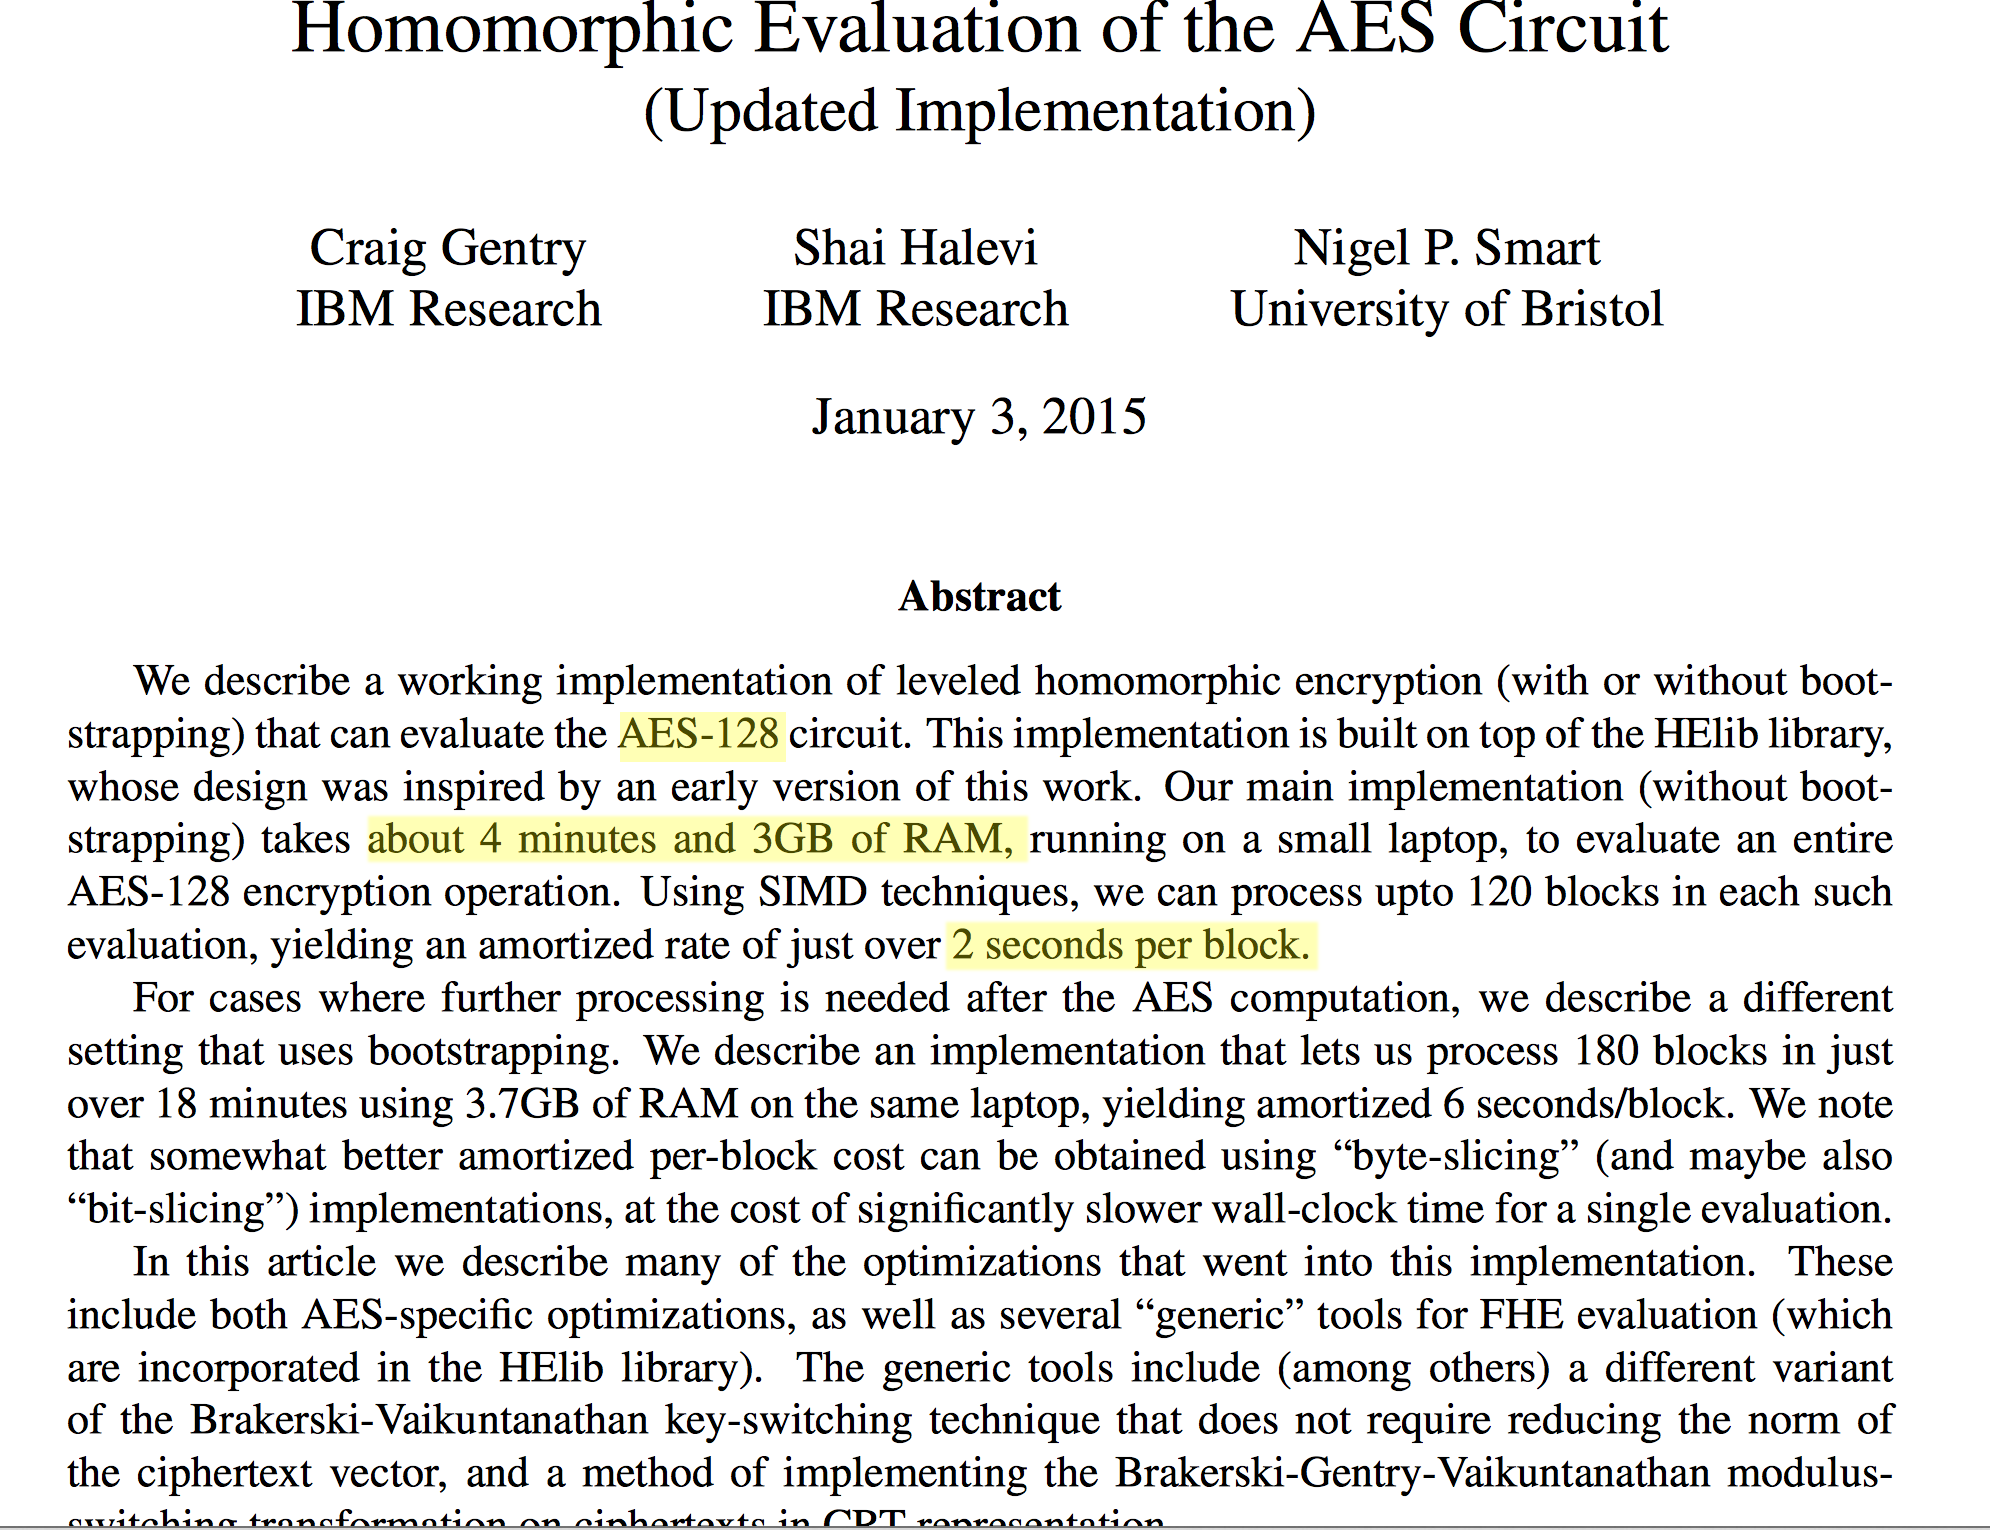
\includegraphics[width=\textwidth]{./pictures/homomorphic-aes}
\end{frame}

\begin{frame}{Conclusion}
	\begin{itemize}
		\item Homomorphic encryption lets us operate on ciphertext and influence
			plaintext
		\item Most schemes work really well for only one operation
		\item FHE is possible, but very slow and rigid
	\end{itemize}
\end{frame}


\begin{frame}{Questions / Comments?}{Please encrypt your question with whatever
	key you like}
\end{frame}

\end{document}
